\section{Spheres}

The standard model is created in Blender using an icosphere with 5 subdivisions. It is centred in the origin with radius r equal to 1.
Then, it is translated by a vector v = (x, y, z) to it is new position and scaled of a given factor in order to match the desired position and dimension. The z-traslation equals to r/2, in order to place the base of the sphere on the floor. This ensures that the nanoparticle rests perfectly on the substrate.
Some examples of generated images are reported in Fig. \ref{fig:sphere}a-c. In particular, Fig. \ref{fig:sphere_b} and \ref{fig:sphere_c} show also compenetrated spheres that are successfully handled by this system.

\begin{figure}[ht]
    \centering
    \begin{subfigure}[b]{0.32\textwidth}
        % sfera_singola
        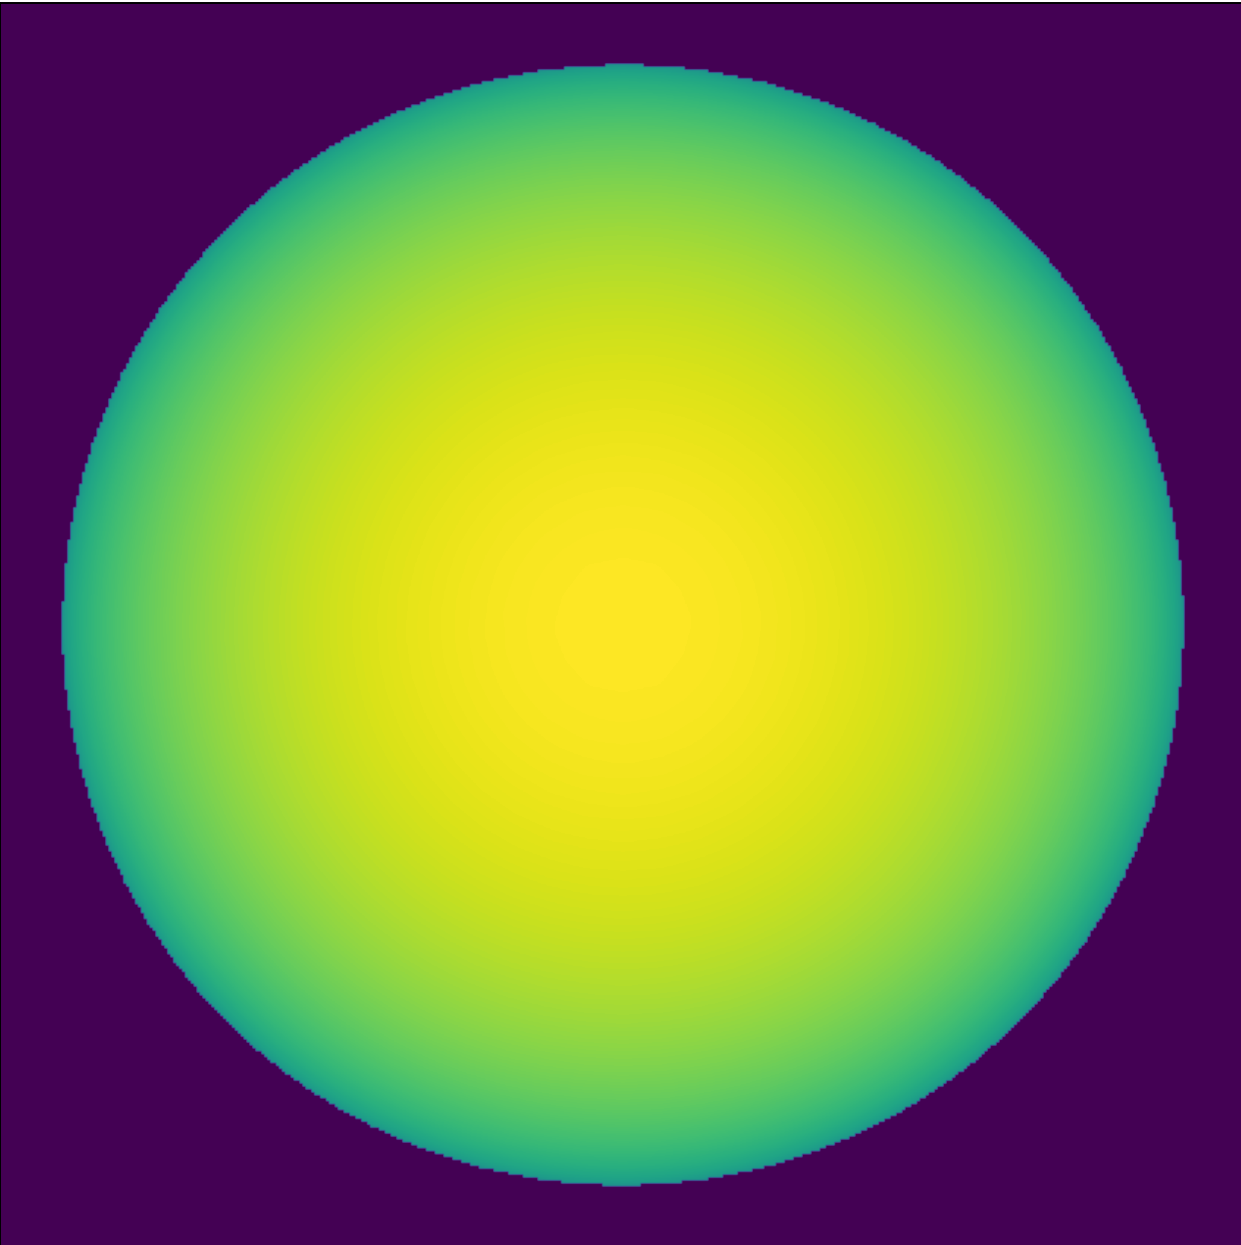
\includegraphics[width=.95\textwidth]{./immagini/sfera_singola.png}
        \caption{}
        \label{fig:sphere_a}
    \end{subfigure}
    \hfill
    \begin{subfigure}[b]{0.32\textwidth}
        % sfera_doppia
        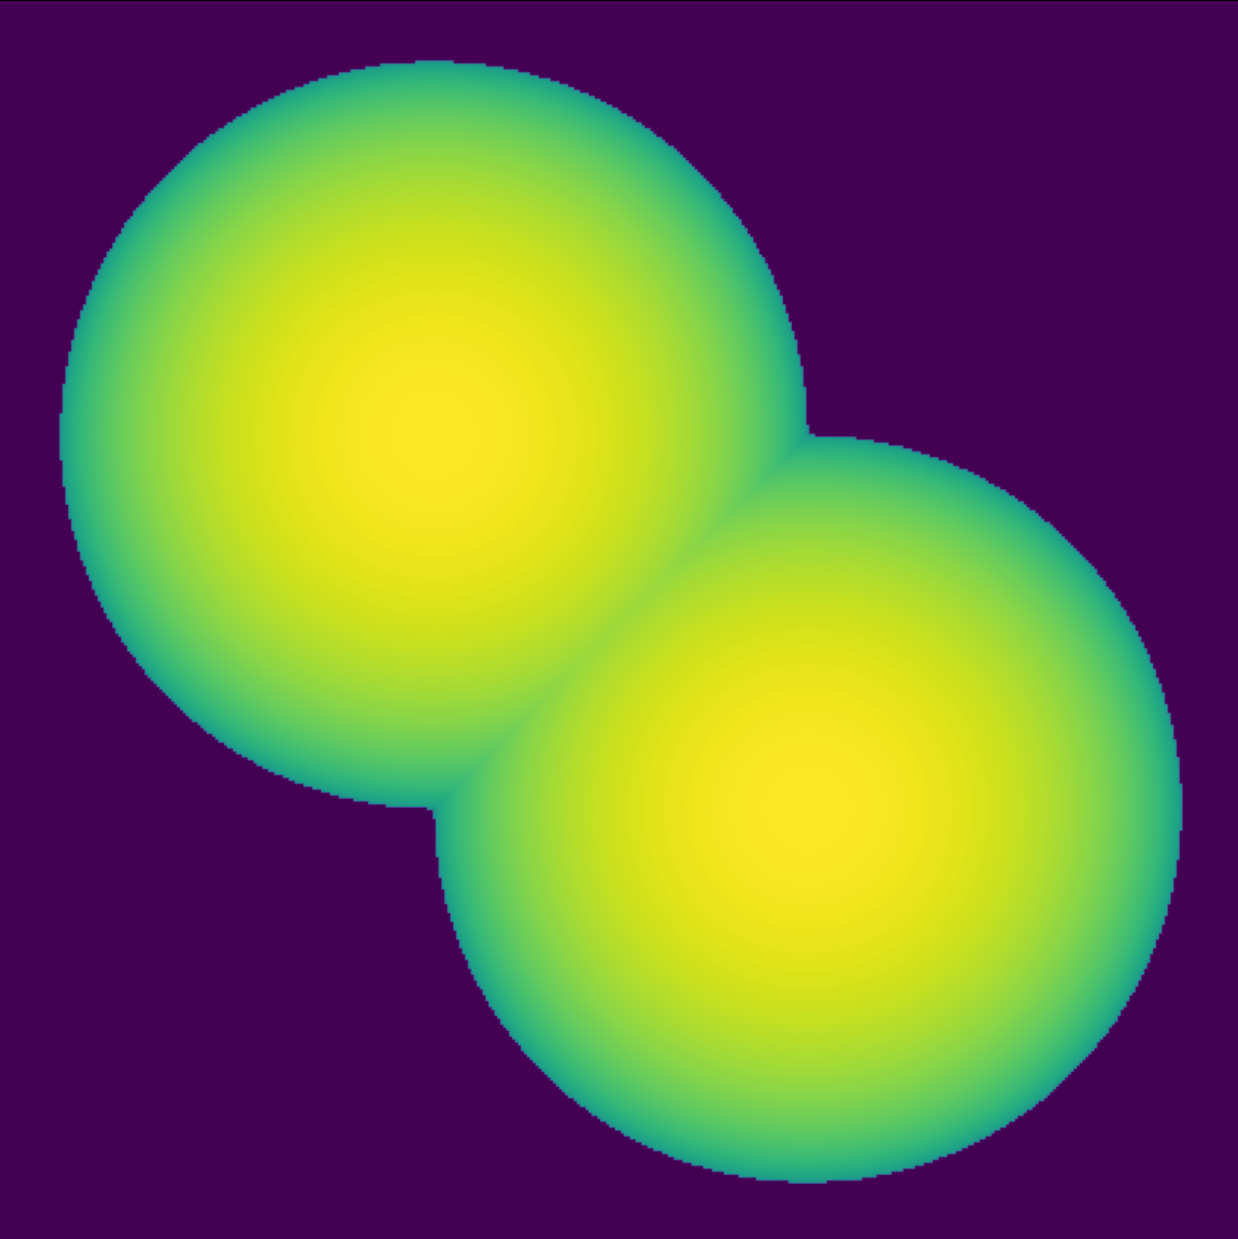
\includegraphics[width=.95\textwidth]{./immagini/sfera_doppia.png}
        \caption{}
        \label{fig:sphere_b}
    \end{subfigure}
    \hfill
    \begin{subfigure}[b]{0.32\textwidth}
        % sfera_statistica
        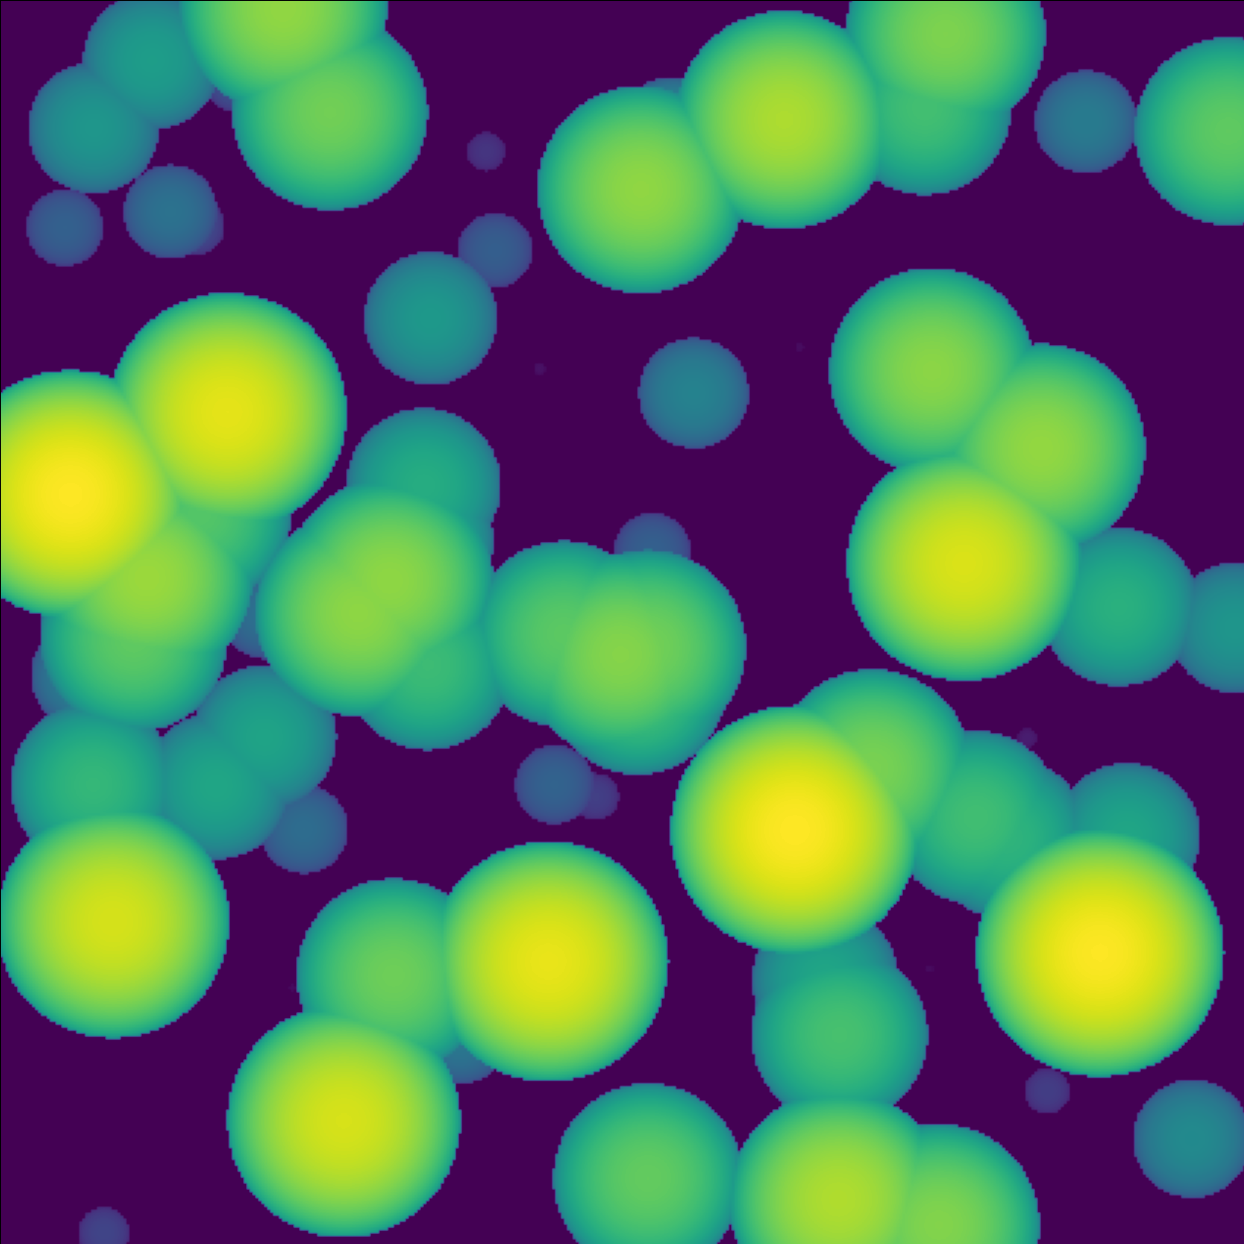
\includegraphics[width=.95\textwidth]{./immagini/sfera_statistica.png}
        \caption{}
        \label{fig:sphere_c}
    \end{subfigure}
    \caption{a) Single, b) Double and  c) Statistic used spheres}
    \label{fig:sphere}
\end{figure}